\subsection{The TSR-tree Index}
\label{sec:tsrtree}

%We first present the structure of our proposed index, the \tsr, and then discuss query evaluation.

\subsection{Index Structure}
\label{subsec:index_structure}

The \tsr is an enhanced R-tree. As in the standard R-tree \cite{Guttman1984}, each node has at least $m$ and at most $M$ entries and stores the MBRs of its children. Additionally, for each child, a node stores a pair of \emph{Minimum Bounding Time Series} (MBTS) that enclose all the time series indexed in its subtree. More specifically, this pair consists of an \emph{upper bounding time series} $T_{up}$ and a \emph{lower bounding time series} $T_{lo}$, respectively constructed by selecting the maximum (for $T_{up}$) and minimum (for $T_{lo}$) of values at each time point among all objects indexed therein. 
Formally, let $\mathcal{T}_N$ denote the set of objects contained in the subtree rooted at entry $N$ of a node. Then, the MBTS of $N$ comprises two (virtual) time series, $T_{N,up}$ and $T_{N,lo}$, which are derived by selecting the maximum and minimum values, respectively, among all the time series in $\mathcal{T}_N$, i.e.:

\begin{align}\label{eq:bounds}
 \begin{split}
  & T_{N,up} = \{ \max_{T \in \mathcal{T}_N} T[0], \ldots, \max_{T \in \mathcal{T}_N} T[w-1] \} \\
  & T_{N,lo} = \{ \min_{T \in \mathcal{T}_N} T[0], \ldots, \min_{T \in \mathcal{T}_N} T[w-1] \}
 \end{split}
\end{align}


%\begin{figure}[!t]
%	\centering
%	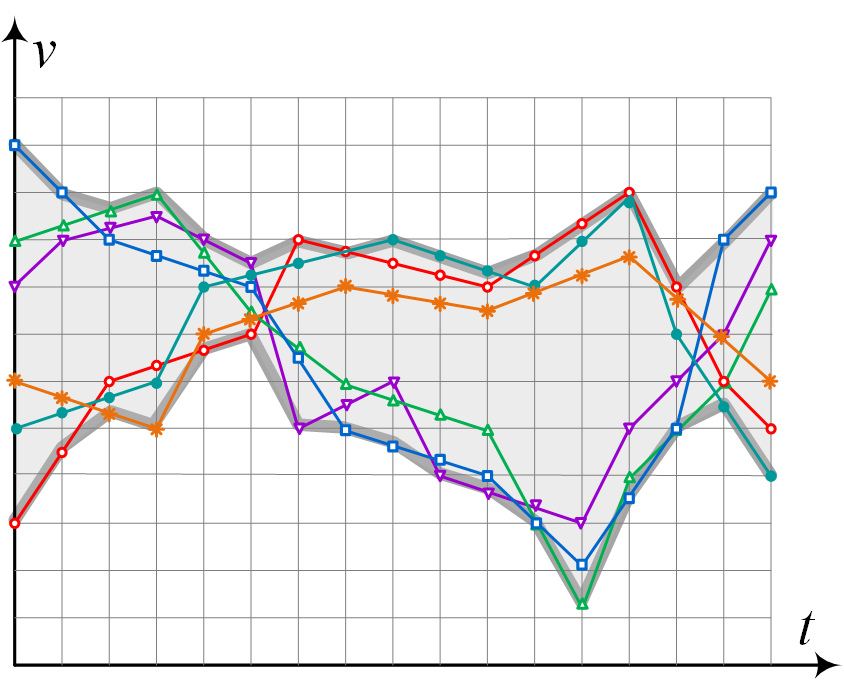
\includegraphics[width=0.8\columnwidth]{figures/bounds_tsr.png}
%	\caption{Example of the MBTS enclosing a set of time series.}
%	\label{fig:tsr_mbts}
%\end{figure}






\begin{myexample}
 Figure \ref{subfig:tsr_mbts} illustrates an example of the MBTS of a set of given time series. The latter are represented in the figure by colored solid lines with different markers. The upper and lower bounding time series are represented by thick grey lines, enclosing the whole (shaded) area where the individual time series lie. \qed
\end{myexample}





%Optionally, as will be explained below, the node may also store for each child a (virtual) average time series (AVTS), $T_{N_i,av}$, which is composed of the average values of all the time series in that child's subtree, i.e.:
%
%\begin{equation}
% T_{N_i,av} = \{ \avg_{T \in \mathcal{T}_{N_i} } T[0], \ldots, \avg_{T \in \mathcal{T}_{N_i} } T[w] \}
%\end{equation}

%Figure \ref{fig:rts_baseline} depicts an \mnote{example (TODO: update)} of the baseline R-TS index. The two small frames on the bottom illustrate the upper and lower time-series bounds. The left frame contains the bounds for node R5, with the darker colored one being the upper and the more gray-ish being the lower bound. The right frame contains the bounds of the node R10. Since this is a child of node R5, its bounds are contained by R5's bounds, outlined with a dashed line.

%\begin{figure}[!t]
% \centering
% %\hspace{-5pt}
% \subfigure[$Q_{bb}(T_q, \theta_{sp}, \theta_{ts})$]{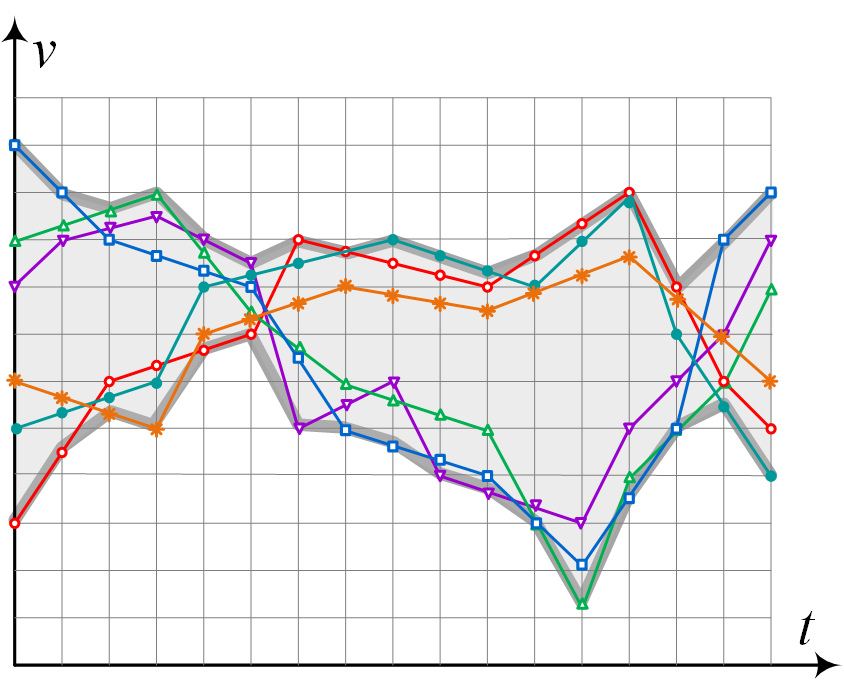
\includegraphics[width=0.235\textwidth]{figures/bounds_tsr.png}\label{subfig:example_queries_bb}}
% %\hspace{-5pt}
% \subfigure[$Q_{kb}(T_q, k, \theta_{ts})$]{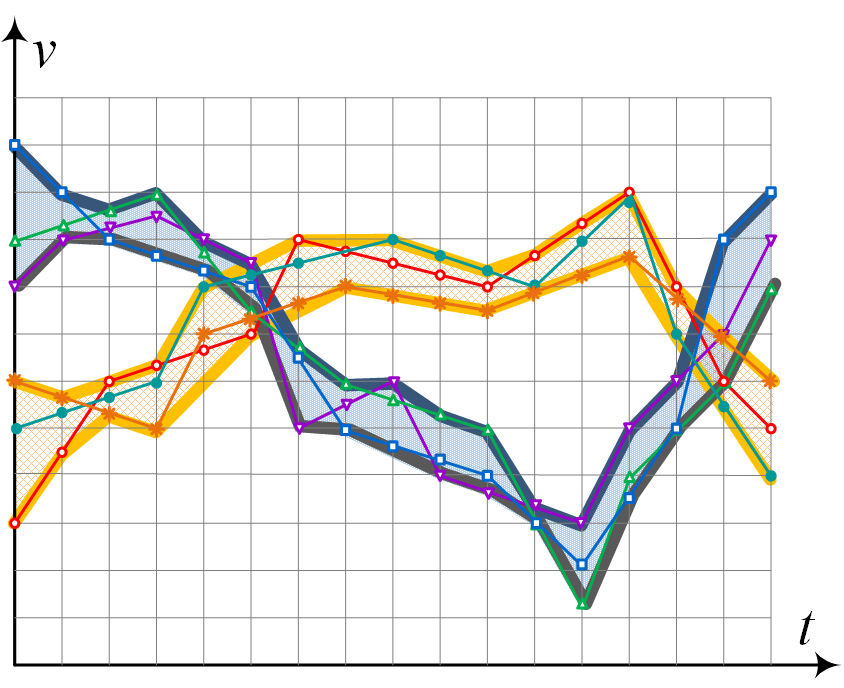
\includegraphics[width=0.235\textwidth]{figures/bounds_ctsr.png}\label{subfig:example_queries_kb}}
% %\vspace{-10pt}
%\caption{An example illustrating hybrid queries on geolocated time series. \mnote{Try to increase sizes of icons and fonts. Also, better replace $Q_{rr}$ and $Q_{kr}$ with just $T_q$ in both cases.}}
%\label{fig:example_queries}
%\end{figure}



%\begin{figure}[!t]
%	\centering
%	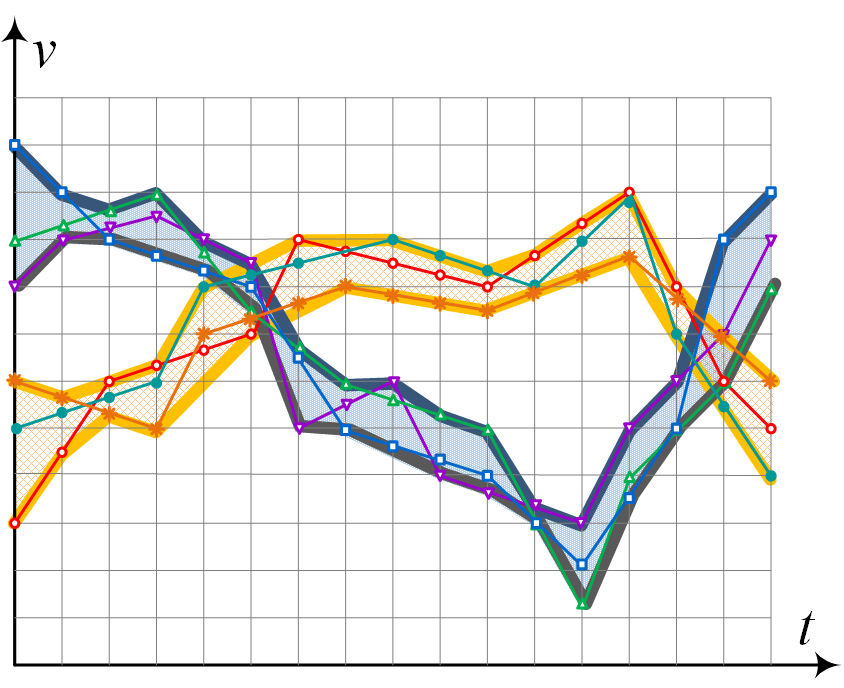
\includegraphics[width=0.8\columnwidth]{figures/bounds_ctsr.png}
%	\caption{A simple example of the baseline version of the R-TS index. Each node has its own time-series bounds.}
%	\label{fig:rts_baseline}
%\end{figure}


%\subsection{Index Construction and Maintenance}
%\label{subsec:index_construction}

Construction and maintenance of the \tsr follow the standard procedures of the R-tree for data insertion, deletion and node splitting. Objects (i.e., geolocated time series) are always inserted into leaves. The difference is that, after the R-tree has been built, it is traversed in a reverse breadth-first manner and the MBTS of each node are calculated. Moreover, the heuristic for determining where each object will be inserted can be adapted to also account for the similarity of objects in the time series domain, in addition to their spatial distance. Recall that in the standard R-tree, selecting the node where a new object will be inserted is based on finding the entry where such an insertion incurs the least possible enlargement of its MBR. Now, this is extended to also consider the enlargement incurred in that entry's MBTS. Specifically, selecting the appropriate node $N$ should minimize the following hybrid cost function:
\begin{equation}
 cost(T, N) = \lambda \cdot cost_{sp}(T, N) + (1 - \lambda) \cdot cost_{ts}(T, N)
 \label{eq:insertion_cost}
\end{equation}

\noindent where $T$ is the new object for insertion, $cost_{sp}$ and $cost_{ts}$ are functions quantifying the cost of enlarging $N$'s MBR and MBTS, respectively, and $\lambda$ is a weight parameter determining the relative importance of the two factors. Notice that for $\lambda = 1$ this heuristic behaves exactly as in the standard R-tree. When checking a given object $T$ for insertion in node $N$, we calculate distance $\delta_i$ between $T$ and current MBTS at each time point $i \in \{ 1, \dots, w \}$:
\begin{equation}
 \begin{split}
  \delta_i = \begin{cases}
	T[i] - T_{N, up}[i], & \text{if} \;\; T[i] > T_{N, up}[i] \\
	T_{N, lo}[i] - T[i], & \text{if} \;\; T[i] < T_{N, lo}[i] \\
	0, & \text{if} \;\; T_{N, lo}[i] \leq T[i] \leq T_{N, up}[i].
	  \end{cases}
 \end{split}
 \label{eq:delta_ts}
\end{equation}

\noindent Such distances $\delta_i$ are shown with dashed red lines in Figure~\ref{subfig:mbts_bounds}. Thus, we can quantify enlargement $cost_{ts} = \sum{\delta_i}$ of MBTS for $N$. 

%\mnote{If it turns out that using the avg is important, we can elaborate here on the calculation of $cost_{ts}$ ...}


\subsubsection{Hybrid Node Pruning}
\label{subsec:index_pruning}

For efficient query execution, the goal is to reduce the number of node accesses by pruning subtrees of the index that cannot contain any results. To do so, we need to establish lower bounds for the different types of distances between the query object $T_q$ and any objects contained in the subtree rooted at a node $N$ in the index. In the spatial domain, this bounding $mindist_{sp}(T_q, N)$ is computed as in the case of the standard R-tree, i.e., based on $N's$ MBR. Similarly, in the time series domain, the corresponding bounding distance is derived by $N's$ MBTS. Following Equations \ref{eq:dist_ts} and \ref{eq:bounds}, it can be easily seen that this can be calculated as follows:
\begin{equation}
 mindist_{ts}(T_q, N) = \frac{\displaystyle \sqrt{\sum_{i=1}^{w} \delta_i^2}}{maxDist_{ts}}, \\
\label{eq:mindist_ts}
\end{equation}

\noindent where $\delta_i$ represents distances between $T_q$ and MBTS at each time point $i$, computed analogously to Equation~\ref{eq:delta_ts}.

%\begin{align}
% \begin{split}
%  & mindist_{ts}(T_q, N) = \frac{\displaystyle \sqrt{\sum_{i=1}^{w} \delta_i^2}}{maxDist_{ts}}, \\
%  & \text{where} \\
%  & \delta_i = \begin{cases}
%	T_q[i] - T_{N, up}[i], & \text{if} \;\; T_q[i] > T_{N, up}[i] \\
%	T_{N, lo}[i] - T_q[i], & \text{if} \;\; T_q[i] < T_{N, lo}[i] \\
%	0, & \text{if} \;\; T_{N, lo}[i] \leq T_q[i] \leq T_{N, up}[i].
%	  \end{cases}
%\end{split}
%\label{eq:mindist_ts}
%\end{align}


\begin{myexample}
  Figure \ref{subfig:mbts_bounds} depicts a query time series (the magenta solid line) and the bounds (thick gray lines) in the MBTS of a node. The vertical dashed red lines outside MBTS indicate distances between the query and those bounds contributing to $mindist_{ts}(T_q, N_i)$.   \qed 
\end{myexample}


%\begin{figure}[ht]
%	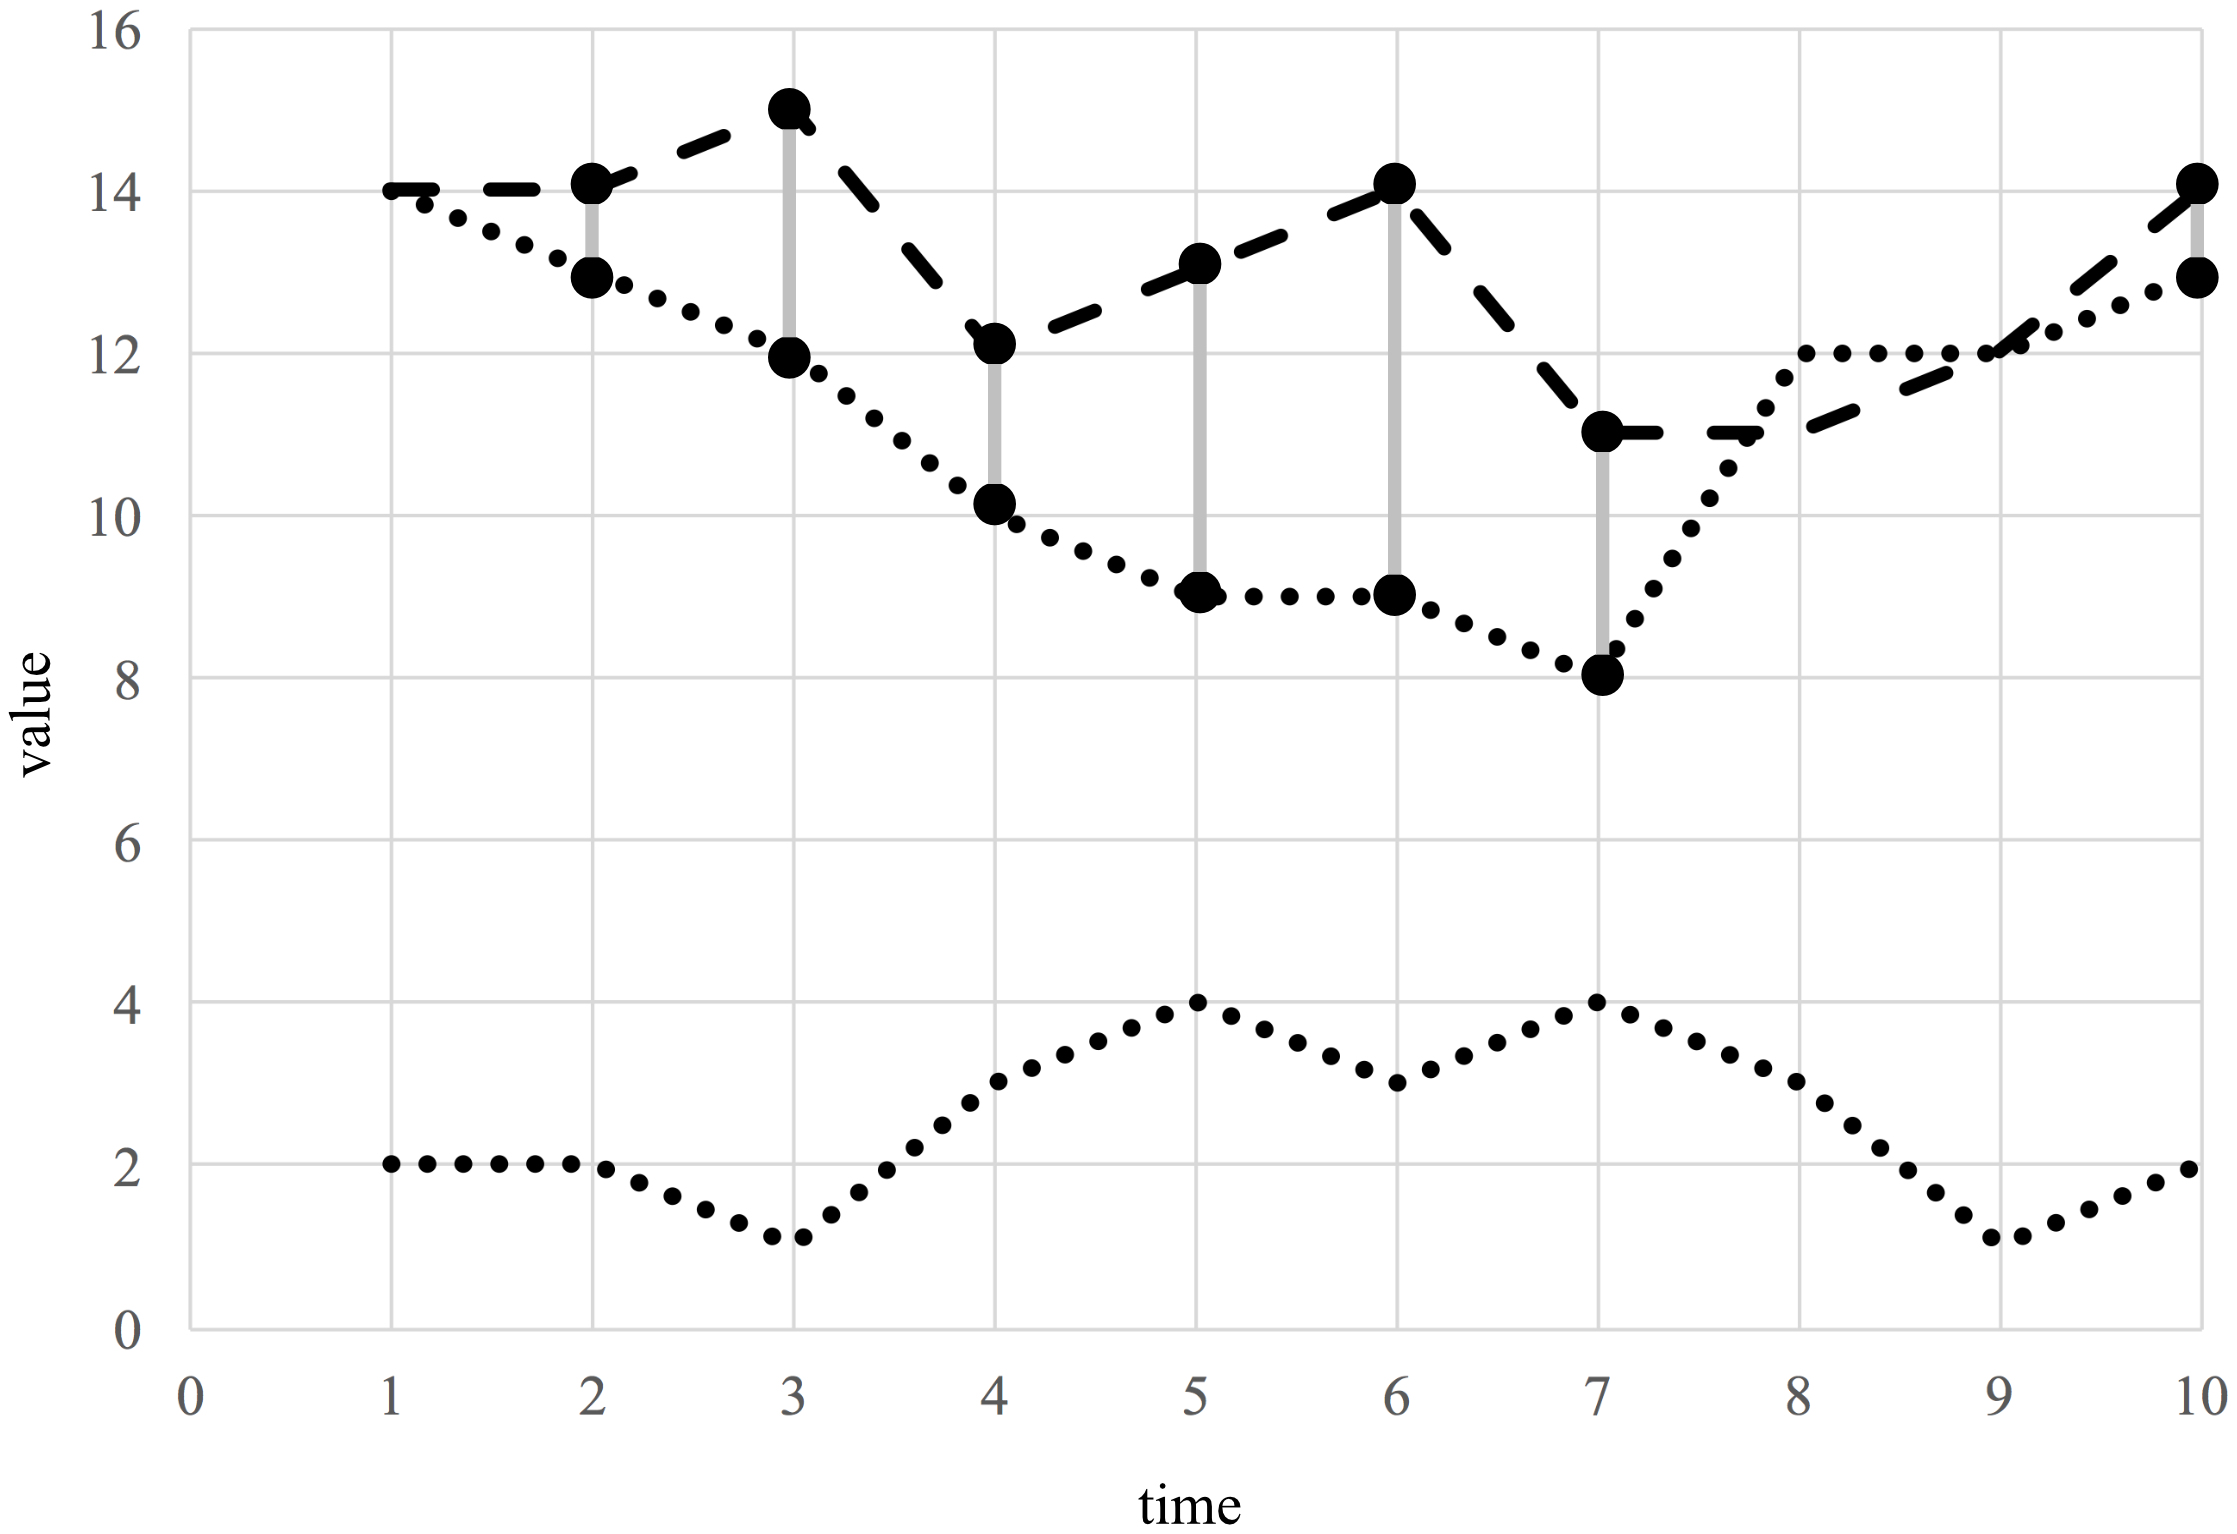
\includegraphics[scale=0.29]{figures/bounds.png}
%	\caption{The distances that contribute to $MINDST_{b}$}
%	\label{fig:bounds}
%\end{figure}


Moreover, given that the objects under a node $N$ are a subset of those of its parent $N'$, it follows from the definition of the time series bounds (Equation \ref{eq:bounds}) that the MBTS of $N$ is tighter than (or equal to) the MBTS of $N'$. From Equation \ref{eq:mindist_ts}, this guarantees that:
\begin{equation}
 mindist_{ts}(T_q, N') \leq mindist_{ts}(T_q, N).
\end{equation}

\noindent So, if $mindist_{ts}(T_q, N')$ is higher than threshold $\theta_{ts}$ specified by the query, the entire subtree rooted at $N'$ can be pruned altogether.

Finally,  from Equations \ref{eq:sim_h} and \ref{eq:dist_h} we can observe that hybrid distance $dist_h(T_q, T)$ is monotone with respect both to $dist_{sp}(T_q, T)$ and $dist_{ts}(T_q, T)$. This implies that a minimum hybrid distance bound $mindist_h(T_q, N)$ for the contents of a given node $N$ can be similarly established by combining the individual bounds $mindist_{sp}\\(T_q, N)$ and $mindist_{ts}(T_q, N)$, i.e.:
\begin{equation}
mindist_h(T_q, N) = 1 - (1 - mindist_{ts}(T_q, N)) \; e^{- \gamma \; mindist_{sp}(T_q, N)}
\end{equation}


\subsubsection{Hybrid Query Processing}
\label{subsec:index_query}


Query processing in \tsr follows a similar procedure to the respective processes for boolean range \cite{Guttman1984} and $k$NN queries \cite{hjaltason99tods} in R-trees. However, this is now extended by utilizing all available bounds $mindist_{sp}$, $mindist_{ts}$ and $mindist_h$, thus pruning nodes simultaneously in the spatial dimension and the time series dimension while traversing the index. This reduces node accesses during evaluation of hybrid queries. Next, we outline the algorithms for executing each of the query variants presented in Section \ref{subsec:query_types}.

\subsubsubsection{$Q_{bb}(T_q, \theta_{sp}, \theta_{ts})$}
\label{subsubsec:double_range}

To evaluate this query, we recursively traverse the \tsr starting from the root. For each node $N$, the following two conditions are checked: (a) $mindist_{sp}(T_q, N) \leq \theta_{sp}$ and (b) $mindist_{ts}(T_q, N) \leq \theta_{ts}$. If either of these conditions returns false, $N$ is pruned. Once a leaf node is reached, the objects (i.e., geolocated time series) contained therein are retrieved, and each one is checked if it qualifies the query criteria. The steps for processing this query are shown in detail in Algorithm \ref{alg:double_range_query}.

\begin{algorithm}[!t]
\begin{small}
	\DontPrintSemicolon
	%\KwIn{Starting node $N$, geo-located query $T$, spatial domain threshold $\theta_{sp}$, time-series domain threshold $\theta_{ts}$}
	%\KwOut{All the geo-located time-series that satisfy the given constraints $res$}
	%\BlankLine
	\Begin{
		$R \leftarrow \emptyset$ \\
		$L \leftarrow$ root entries \\
		\While{$L \neq \emptyset$}{
			$N \leftarrow L.getNext()$ \\
			\If{$N$ is not leaf}{
				\ForEach{$N' \in N.getChildren()$}{
					\If{$mindist_{sp}(T_q, N') \leq \theta_{sp}$ $\land$ $mindist_{ts}(T_q, N') \leq \theta_{ts}$}{
						$L \leftarrow L \cup \{ N'.getChildren() \}$ \\
%						$res \leftarrow res \cup DoubleRange(C, T, \theta_{sp}, \theta_{ts})$ \\
					}
				}
				%$return(res)$
			}
			\Else{
				\ForEach{$T \in N.getObjects()$}{
					\If{$dist_{sp}(T_q, T) \leq \theta_{sp} \land dist_{ts}(T_q, T) \leq \theta_{ts}$}{
						$R \leftarrow R \cup \{ T \}$ \\
					}
				}
				$return(R)$
			}
		}
	}
	\caption{$Q_{bb}(T_q, \theta_{sp}, \theta_{ts})$}
	\label{alg:double_range_query}
\end{small}		
\end{algorithm}


\subsubsubsection{$Q_{kb}(T_q, k, \theta_{ts})$ and $Q_{bk}(T_q, \theta_{sp}, k)$}
\label{subsubsec:range_topk}

These queries combine a boolean filter and a top-$k$ filter. To retrieve top-$k$ results, we employ a \textit{best-first search} approach using a priority queue, as in a typical best-first traversal algorithm \cite{hjaltason99tods}.

Assume that we are evaluating a $Q_{bk}(T_q, \theta_{sp}, k)$ query. Initially, the root entries are retrieved, and their lower spatial distance bound $mindist_{sp}$ is calculated. For a given such entry, if its  $mindist_{sp}\geq\theta_{sp}$, then the underlying subtree can be safely pruned. Otherwise, this entry's $mindist_{ts}$ is calculated, and the entry is pushed to the priority queue according to its $mindist_{ts}$ value in ascending order. The process continues recursively, pulling the next item from the queue. If this is a leaf, we retrieve all its objects, calculate their exact spatial distances $dist_{sp}$, and the ones that are not filtered out are pushed to the queue, based on their $mindist_{ts}$. If a pulled item is an object (i.e., geolocated time series), we add it to the result set. The process terminates once $k$ results have been retrieved. Algorithm \ref{alg:range_topk_query} describes the above procedure in more detail. 

Evaluating a $Q_{kb}(T_q, k, \theta_{ts})$ is straightforward; the treatment of the spatial and the time series dimensions is simply reversed.

%At first, we initialize list of final results and insert the root of the index in the priority queue (Lines 2-3). Then, while the queue is not empty (Line 4), we poll the top element (Line 5) and check whether it is am inner node, a leaf node, or a raw geo-located time-series object. In the first case, we obtain its children nodes, and for each one we calculate the distance of its MBR to the query (Lines 16-18). If the distance is less than $\theta_{sp}$ (Line 19), we calculate the $MINDIST_{b}$ distance of the node to the query and add the child to the queue. In case it is a leaf node, we obtain all its children (i.e., raw geo-located time-series) and for each one we calculate its Euclidean time-series distance to the query and add it to the queue (Lines 12-15). Finally, if the element is a raw object, calculate its distance to the query and if it is less than the threshold $\theta_{sp}$ add it to the final results (Lines 6-9). If the size of the final result list becomes equal to $k$, break and return the list (Lines 10-11 and 22).

\begin{algorithm}[!t]
\begin{small}
	\DontPrintSemicolon
	%\KwIn{Root $R$, geo-located query $T$, spatial domain threshold $\theta_{sp}$, number of desired results $k$}
	%\KwOut{All the geo-located time-series that satisfy the given constraints $res$}
	%\BlankLine
	\Begin{
		$R \leftarrow \emptyset$ \\
		$Queue \leftarrow$ root \\
%		$topkQ \leftarrow topkQ \cup R$ \\
		\While{$Queue$ is not empty}{
			$X \leftarrow Q.pull()$ \\
			\If{$X$ is a time series}{
%				$dist_{sp} \leftarrow dist_{sp}(T.loc, m.loc)$ \\
%				\If{$dist_{sp} \leq \theta_{sp}$}{
					$R \leftarrow R \cup \{ X \}$ \\
%				}
				\If{$|R| = k$}{
					$break$ \\
				}
			}
			\ElseIf{$X$ is leaf node}{
				\ForEach{$T \in X.getObjects()$}{
					\If{$dist_{sp}(T_q, T) \leq \theta_{sp}$}{
					 $T.dist \leftarrow dist_{ts}(T_q, T)$ \\
					 $Queue.push(T, T.dist)$ \\					 
					}					
%					$el.dist \leftarrow dist_{ts}(T, el)$ \\
%					$topkQ \leftarrow topkQ \cup el$ \\
				}
			}
			\Else{
				\ForEach{$N \in X.getChildren()$}{
					\If{$mindist_{sp}(T_q, N) \leq \theta_{sp}$}{
						$N.dist \leftarrow mindist_{ts}(T_q, N)$ \\
						$Queue.push(N, N.dist)$ \\	
					}
				}
			}
		}
		$return(R)$
	}
	\caption{$Q_{bk}(T_q, \theta_{sp}, k)$}
	\label{alg:range_topk_query}	
\end{small}	
\end{algorithm}


%The algorithm proceeds as follows ... (\mnote{TODO: elaborate}).
%
%It maintains two priority queues, $Res$ and $Visit$. The former has fixed size $k$ and holds the current result set (i.e., raw time series) sorted in increasing order of $dist_{ts}$. The latter holds node entries (i.e., elements $N_i$) sorted in increasing order of $mindist_{ts}$. Initially, $Res$ is empty, and $Visit$ is initialized with the root of the \tsr index. The algorithms also keeps track of the current distance threshold in the time series domain, $\theta_{ts}$, which is always set to be equal to the distance of the $k$-th time series in $Res$ to the query time series $T_q$. While $|Res| < k$, $\theta_{ts,k}$ is set to infinite (or null).
%
%At each step, the algorithm dequeues the top element (i.e., tree node) from $Visit$. If it is an internal node, it retrieves its entries. For each entry $N_i$, it first checks whether $mindist_{sp}(T_q, N_i) \leq \theta_{sp}$. If not, $N_i$ is pruned. Otherwise, it checks whether $mindist_{ts}(T_q, N_i) \leq \theta_{ts}$. Again, if not, $N_i$ is pruned. Otherwise, $N_i$ is inserted in $Visit$. If it is a leaf node, the time series contained in it are retrieved. For each one, we first check its spatial distance, and if it is not pruned, we check its time series distance. If the latter is lower than $\theta_{ts}$, it is inserted in $Res$, and $\theta_{ts}$ is updated accordingly.
%
%The process terminates when the top element of $Visit$ has $mindist_{ts}(T_q, N_i)$ $>$ $	\theta_{ts}$ or when $Visit = \emptyset$.


%Finally, the $k$NN range query's functionality is similar to the Range-Top-$k$ query described above, with the difference that in this case the priority queue is based on the spatial distance instead of the time series distance, and the pruning is applied on the spatial domain instead of the time-series domain.


\subsubsubsection{$Q_{hb}(T_q, \theta_h, \gamma)$ and $Q_{hk}(T_q, k, \gamma)$}
\label{subsubsec:hybrid_range_query}

These queries apply a boolean and a top-$k$ filter, respectively. In both cases, this is applied on the hybrid distance $dist_h(T_q, T)$ of the query object $T_q$ to each of the candidate objects $T$.

For $Q_{hb}(T_q, \theta_h, \gamma)$, query evaluation follows the same process as outlined in Algorithm \ref{alg:double_range_query}. The difference is that instead of checking separately the given distance thresholds on the spatial and the time series distances, a single check is made comparing the hybrid distances $dist_h$ and $mindist_h$ against the single threshold $\theta_h$.

Evaluation of the $Q_{hk}(T_q, k, \gamma)$ query is similar to the one outlined in Algorithm \ref{alg:range_topk_query}. In this case the difference is that there is no boolean filtering involved, so objects and nodes are inserted into the priority queue according to their hybrid distance, $dist_h$ and $mindist_h$, respectively. Again, the algorithm terminates once $k$ objects are pulled from the queue; these are the top-$k$ results.

%\mnote{Essentially, we just need to state that for the hybrid mindist it also holds that the mindist of a child node is at least as high as that of the parent node, and hence pruning and best first search works accordingly...}

%The hybrid range query operates on the hybrid distance (Equation \ref{eq:4}) described in Section \ref{subsec:preliminaries}. We initially recursively traverse the index, taking under consideration only the nodes whose hybrid distance to the query is less than $\theta_{hb}$. The hybrid distance between an inner node and the query is calculated by replacing in Equation \ref{eq:4} the spatial distance with the distance between the query and the node's MBR and the time-series distance with the $MINDST_{b}$ distance between the node's bounds and the query:

%and has the following format:
%\begin{equation} \label{eq:10}
%	Q_{hrange} = \{q, \theta_{hb}\}
%\end{equation}
%where $q$ is the query as a geo-located time-series and $\theta_{hb}$ is a hybrid distance threshold that has to be satisfied in order to accept an element as part of the answer.


%\begin{equation} \label{eq:11}
%	\begin{split}
%		dist_{hb}(T, N) = \lambda \cdot \frac{dist_{sp}(T.loc, N.mbr)}{maxD_{sp}} + \\ + (1-\lambda) \cdot \frac{MINDST_{b}(T, N^{b}_{u}, N^{b}_{l})}{maxD_{ts}}
%	\end{split}
%\end{equation}
%
%where $T.loc$ is the spatial part of the query, $N.mbr$ is the current node's MBR and $N^{b}_{u}, N^{b}_{l}$ are the node's upper and lower bounds recursively. Upon reaching a leaf, the hybrid distance of each element it contains to the query is calculated and only the ones that satisfy the threshold $\theta_{hb}$ are added to the results. 

%Finally, the hybrid top-$k$ query makes use of the best-first search approach, each time traversing the node that is closer to the query in terms of the hybrid distance in Equation \ref{eq:11}. The query starts from the root node, adding all its children to a priority queue that keeps them sorted according to the hybrid distance. Then at each iteration, it polls an element from the queue and, if it is an inner-node, it similarly adds its children to the queue. If it is a leaf node, it obtains its raw geo-located time-series, calculates their hybrid distance using Equation \ref{eq:4} and adds the top-$k$ of them to the top-k queue via a local queue. When, during an iteration, a raw geo-located time-series is polled from the queue, it is added to the final results. When the size of the results reaches $k$, the results are returned. This way, the remaining unexplored nodes in the queue do not need to be traversed and are thus, pruned. 


\subsection{The BTSR-tree Index}
\label{sec:ctsrtree}

%\subsection{Index Description}
%\label{subsec:index_descr}

%In Section \ref{sec:related} we described a number of state-of-the-art hybrid index techniques for spatio-textual data. To our knowledge, currently, there exists no similar hybrid index for annotated time-series data.

%In this section we present how the \textit{R-TS} index is constructed and delineate the way the supported queries are elaborated. R-TS takes advantage of the versatility and space efficiency of the R-Tree and is capable of indexing geo-located time-series of various formats (i.e., normalized, or compressed).

%The annotated time-series are inserted in the R-Tree through a modified cost computation method, that takes under consideration the cost in time-series domain of an insertion, apart from the cost in the spatial domain.

%To allow pruning during executing the queries, we add the proper upper and lower bounds of the time series contained in each node's subtree and introduce a lower bounding distance, thus, eliminating the false negatives.

%\subsubsection{Baseline R-TS Index}
%\label{subsubsec:baseline_rts}
%We first describe a baseline implementation of the proposed index with less tight bounds in the time-series domain. R-TS is consisted of a modified R-Tree that is built by taking into account insertion costs in both spatial and time-series domains.

%Based on the hybrid distance described in Section \ref{subsec:preliminaries}, we define a \textit{hybrid cost function}, that describes the hybrid cost of inserting a geo-located time-series into a node's sub-tree:
%
%\begin{equation} \label{eq:5}
%	\begin{split}
%		cost_{hb}(T, N) = \lambda \cdot \frac{cost_{sp}(T, N)}{parentArea} + \\ + (1-\lambda) \cdot \frac{dist_{ts}(T,N)}{maxParentD_{ts}}
%	\end{split}
%\end{equation}

%where $T$ is a geo-located time-series, $N$ is a node in the index, $\lambda \in [0,1]$ is a weighting parameter determining the relative importance of each individual domain, $cost_{sp}$ is the spatial expansion cost in the node and $dist_{ts}$ is the distance between the time-series that is inserted and the average time-series of all the data that are contained in the node's sub-tree. We normalize the spatial cost with $parentArea$, which is node's $N$ parent's total MBR area. Similarly, we normalize the time distance with $maxParentD_{ts}$, the maximum possible time-series distance achievable within the $N$'s parent's bounds. This cost function ensures that similar annotated time-series in both domains (according the weight factor $\lambda$), will tend to end up in a closer sub-tree, allowing a more efficient pruning during querying.

%Each node of the baseline version holds the following information:
%
%\begin{itemize}
%	\item An MBR of all its sub-trees in the spatial domain.
%	\item The average time-series of all the data contained in its sub-trees.
%	\item An upper time-series bound of the data contained in its sub-trees.
%	\item A lower time-series bound of the data contained in its sub-trees.
%\end{itemize}
% 
%The upper and lower time-series bounds are the maximum and minimum values of all the time-series that can be found in a node's sub-tree and are updated accordingly for each node upon the insertion of a time-series:

%When the algorithm picks a node for insertion, its upper and lower bounds are updated. This way, the bounds will be less tight in the upper levels of the tree and will get tighter as we traverse it. Also, each node's bounds will contain the bounds of its sub-trees.


%The construction of baseline R-TS is performed as follows. The geo-located time-series are fetched from disk in a Comma-Separated Values (CSV) format and inserted in the index using the hybrid cost function \ref{eq:5}. During insertion, we recursively choose the sub-tree that, accepting the annotated time-series, would cost less. For normalization, we keep the maximum and minimum coordinates in each spatial dimension and the maximum and minimum values in the time-series domain. Upon choosing a specific sub-tree for the insertion, we update its parent node accordingly:

%\begin{itemize}
%	\item Update its MBR.
%	\item Update its average time-series.
%	\item Update the upper and lower bounds of its sub-tree's time-series.
%\end{itemize}

%When reaching a leaf in the modified R-Tree, the geo-located time-series are stored in a list in memory. If the predetermined maximum number of elements in a leaf node is exceeded, the leaf splits similarly to the R-Tree, but also according to the cost function \ref{eq:5}. The procedure is described in Algorithm \ref{alg:build_index}. More specifically, after initializing the index's root in Line 2, for each geo-located time-series we choose the proper leaf (Lines 3-4) through a modified \texttt{chooseLeaf} method that is described below. Then we insert the geo-located time-series into the index (Line 5). If the leaf's size exceeds the maximum possible (Line 6) we split the leaf node (Line 7) and adjust the index, propagating splits upwards (Line 8). Splitting is performed by a modified \texttt{splitNode} method that operates similarly to the original R-Tree, but using the hybrid cost function \ref{eq:5} instead of the original one. The splitting seed nodes are picked by either R-Tree's \texttt{QuadraticPickSeeds} (also similar to the original R-Tree but using the hybrid cost function), or a modified version of \texttt{LinearPickSeeds}, which will be described later. Similarly, adjusting the tree is performed by a modified (using the hybrid cost function) \texttt{adjustTree} method, that recursively performs any inner necessary splits and updates the proper data (MBR, average time-series and bounds).

%\begin{algorithm}[ht]
%	\DontPrintSemicolon
%	\KwIn{Geo-located time-series dataset $geoTs$, parameter $\lambda$, max node entries $p$}
%	\KwOut{The hybrid index's $root$}
%	\BlankLine
%	\Begin{
%		$R \leftarrow initializeRoot()$ \\
%		\For{$i=1,...,geoTs.size$}{
%			$L \leftarrow chooseLeaf(R, geoTs_{i}, \lambda)$ \\
%			$insertInto(L, geoTs_{i})$ \\
%			\If{$L.size > p$}{
%				$splits \leftarrow splitNode(L, \lambda)$ \\
%				$adjustTree(splits, \lambda)$ \\
%			}
%			\Else{
%				$adjustTree(L, \lambda)$ \\
%			}
%		}
%		$return(R)$
%	}
%	\caption{buildIndex($geoTs$, $\lambda$, $p$, $w$)}
%	\label{alg:build_index}	
%\end{algorithm}

%The modified \texttt{chooseLeaf} method is described in Algorithm \ref{alg:choose_leaf} and operates as follows. It starts from the root node, updating its average time-series data according to the geo-located time-series that is being inserted (Line 2). Its recursion ends when a leaf is reached (Lines 3-4). The minimum found cost is set to a really high number (Line 5), and for each input node's child (Line 6), the hybrid cost is calculated (Line 7), compared with the minimum found cost and if it's smaller, the minimum cost is updated and the current child is set as the selected node (Lines 6-10). Finally, the method recursively calls itself with the selected node as input (Line 11).

%\begin{algorithm}[ht]
%	\DontPrintSemicolon
%	\KwIn{Starting node $N$, geo-located time-series $geoTs$, hybrid cost lambda parameter $\lambda$}
%	\KwOut{Leaf node $L$}
%	\BlankLine
%	\Begin{
%		$N.updateTS(geoTs)$ \\
%		\If{$N.leaf$}{
%			$return(N)$ \\
%		}
%		$minCost \leftarrow Inf$ \\
%		\ForEach{$C \in N.children$}{
%			$cost \leftarrow getHybridCost(C, geoTs, \lambda)$ \\
%			\If{$cost < minCost$}{
%				$minCost \leftarrow cost$ \\
%				$P \leftarrow C$ \\
%			}
%		}
%		$return(chooseLeaf(P, geoTs, \lambda))$
%	}
%	\caption{chooseLeaf($N$, $geoTs$, $\lambda$)}
%	\label{alg:choose_leaf}	
%\end{algorithm}

%\begin{algorithm}[ht]
%	\DontPrintSemicolon
%	\KwIn{Node to be split $N$, hybrid cost lambda parameter $\lambda$}
%	\KwOut{Array of split nodes $splits[]$}
%	\BlankLine
%	\Begin{
%		$cList \leftarrow N.children$ \\
%		$splits[] \leftarrow lPickSeeds(cList)$ \\
%		\While{$!cList.empty$}{
%			$C \leftarrow cList.pop$ \\
%			$cost1 \leftarrow getHybridCost(splits[1], C, \lambda)$ \\
%			$cost2 \leftarrow getHybridCost(splits[2], C, \lambda)$ \\
%			\If{$cost1 > cost2$}{
%				$addChild(splits[1], C)$
%			}
%			\Else{
%				$addChild(splits[2], C)$
%			}
%		}
%		$return(splits[])$
%	}
%	\caption{splitNode($L$, $\lambda$)}
%	\label{alg:split}	
%\end{algorithm}

%In a Big Data scenario, the maximum number of elements that each R-Tree node holds will be significantly larger. Consequently, choosing the appropriate seed when splitting the nodes would be extremely inefficient using the R-Tree's \texttt{QuadraticSplit} algorithm. To provide better scalability, we use a modified version of the \texttt{LinearPickSeeds} function, that properly adapts to the hybrid nature of the data. The idea is to obtain the elements with the highest low rectangle side and lowest high rectangle side, similarly to the original \texttt{LinearPickSeeds}, but with an alteration: For each dimension, i.e., 2 in our case, we seek the maximum high and minimum low coordinate with the highest and lowest possible time-series vector length (average time-series when splitting inner nodes). This way we obtain at most $numDims \cdot 4$ candidate nodes, which are then passed to the modified \texttt{QuadraticPickSeeds} method, which returns the best split seeds. Due to the fixed number of candidate nodes, the \texttt{QuadraticPickSeeds}'s cost is negligible. 

%Algorithm \ref{alg:hybrid_linear_pick_seeds}, outlines the way this function operates. After properly initializing the candidate set (Line 2) the maximum upper and lower bound (Line 4) and the maximum and minimum upper and lower vector lengths (Lines 5-6), we seek to find the following elements: the one with the highest lower side value and highest upper time-series vector length, the one with the highest lower side value and lowest time-series vector length, the one with the lowest high side value and highest upper time-series vector length and the one with the lowest high side value and lowest upper time-series vector length (Lines 7-23). This procedure is repeated for each dimension (Line 3). Finally, the best pair is determined via the \texttt{qPickSeeds} method and returned (Line 24).

%\begin{algorithm}[ht]
%	\DontPrintSemicolon
%	\KwIn{A list of nodes $nList$}
%	\KwOut{A best pair of seed nodes $bestPair$}
%	\BlankLine
%	\Begin{
%		$candidates \leftarrow \emptyset$ \\
%		\For{$i=1,...,numDims$}{
%			$minUb \leftarrow Inf; maxLb \leftarrow -Inf$ \\
%			$maxUvl \leftarrow 0; maxLvl \leftarrow 0$ \\
%			$minUvl \leftarrow Inf; minLvl \leftarrow Inf$ \\
%			\ForEach{$N \in nList$}{
%				\If{$N.Lc_{i} > maxLb \land N.TSvl > maxLvl$}{
%					$maxLvl \leftarrow N.TSvl$ \\
%					$maxLb \leftarrow N.Lc_{i}$ \\
%					$candidates \leftarrow candidates \cup N$
%				}
%				\If{$N.Lc_{i} > maxLb \land N.TSvl < minLvl$}{
%					$minLvl \leftarrow N.TSvl$ \\
%					$maxLb \leftarrow N.Lc_{i}$ \\
%					$candidates \leftarrow candidates \cup N$
%				}
%				\If{$N.Uc_{i} < minUb \land N.TSvl > maxUvl$}{
%					$maxUvl \leftarrow N.TSvl$ \\
%					$minUb \leftarrow N.Uc_{i}$ \\
%					$candidates \leftarrow candidates \cup N$
%				}
%				\If{$N.Uc_{i} < minUb \land N.TSvl < minUvl$}{
%					$minUvl \leftarrow N.TSvl$ \\
%					$minUb \leftarrow N.Uc_{i}$ \\
%					$candidates \leftarrow candidates \cup N$
%				}
%			}
%		}
%		$return(qPickSeeds(candidates))$
%	}
%	\caption{lPickSeeds($nList$)}
%	\label{alg:hybrid_linear_pick_seeds}	
%\end{algorithm}

As explained in the previous section, each node in the \tsr holds an MBTS (i.e., a pair of upper and lower bounding time series) that encloses all the time series contained in its subtree. This allows to prune nodes while traversing the index by computing lower bounds for similarity in the time series domain. Clearly, the pruning effectiveness depends on the tightness of these bounds.

%The shortcoming of the \tsr lies in the fact that, since there is no guarantee that the time series contained in the same node entry will be highly similar to each other, these bounds are typically expected to not be sufficiently tight. Furthermore, constructing these aggregate time series bounds from a set of dissimilar time series, results in bounding time series that are not very similar to any of the enclosed ones. These observations are also obvious in the example of Figure \ref{subfig:tsr_mbts}, where the constructed MBTS encloses a much larger area (shown in grey) than the one actually occupied by the contained time series, and the resulting bounding time series do not closely resemble any of the original ones.


The \tsr does not provide any explicit guarantee that time series contained in the same node are highly similar to each other, hence the produced bounds are typically expected not to be sufficiently tight. Further, constructing the aggregate bounds from a set of dissimilar time series, yields bounding time series that are not very similar to any of the enclosed ones. These observations are obvious in the example of Figure \ref{subfig:tsr_mbts}, where the constructed MBTS encloses a much larger (grey shaded) area than the one actually occupied by the contained time series, and the resulting bounding time series do not closely resemble any of the original ones.

To overcome this issue, we present an optimized version of the \tsr, which we call \ctsr. In a nutshell, the idea is to \emph{bundle} similar time series together in each node, and construct individual MBTS per bundle. This allows to derive bounding time series that are tighter and resemble more closely the enclosed ones. 

%\begin{figure}[!t]
%	\centering
%	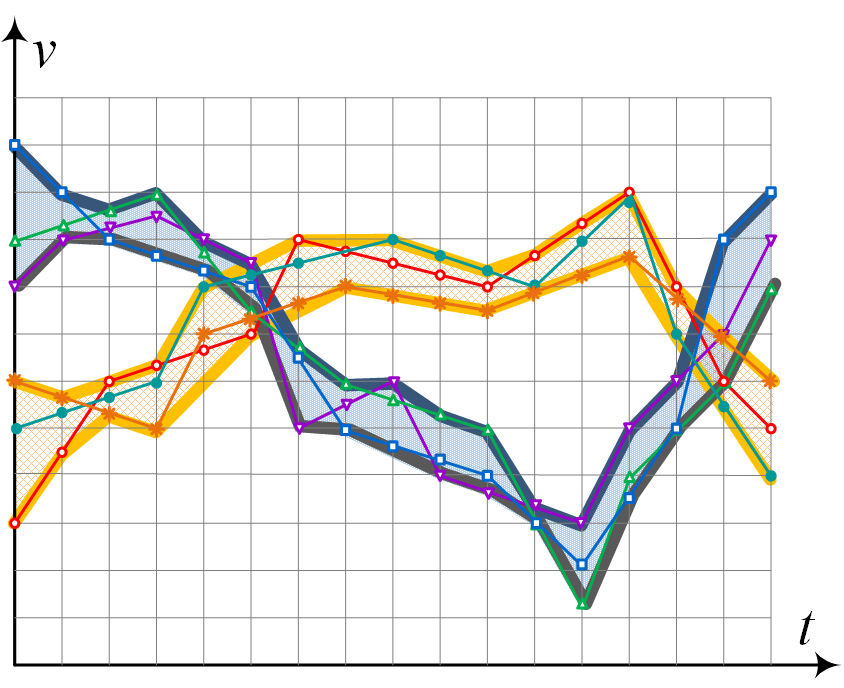
\includegraphics[width=0.8\columnwidth]{figures/bounds_ctsr.png}
%	\caption{Example of the MBTS enclosing a set of \emph{bundled} time series.}
%	\label{fig:ctsr_mbts}
%\end{figure}

\begin{myexample}
 Figure \ref{subfig:btsr_mbts} illustrates this idea using the same example as Figure \ref{subfig:tsr_mbts}. The original time series are now grouped in two bundles, and the MBTS of each bundle is constructed separately. The resulting bounds are now much tighter, eliminating much of the dead space within the MBTS and allowing more precise similarity comparisons.
\end{myexample}


The \ctsr index is built similarly to the \tsr index. To construct the time series bundles within each node, we rely on $k$-{\em means clustering}. To avoid confusion with the top-$k$ predicate in queries, next we symbolize with $\beta$ is the number of bundles to be created. The process is performed bottom-up, starting from the leaf nodes of the index. In each leaf node, the contained time series are clustered into $\beta$ bundles. Then, the MBTS of each bundle is computed and stored in the node. Each internal node receives all the MBTS of its children so as to compute its own $\beta$ bundles and respective set of MBTS. Thus, the process propagates upwards, until reaching the root of the tree.

The higher the number $\beta$ of bundles, the tighter the resulting bounds. But this also implies that a larger number of MBTS needs to be maintained within each node. Hence, the number of bundles that can be created is limited by node capacity. Another observation is that as we move from the leaf nodes to the root, a higher number $\beta$ of bundles is needed, since nodes become increasingly more heterogeneous in the time series they contain in their subtree.

To address such issues, we increase the number of bundles bottom-up at every tree level by a factor $c$. Hence, a node at level $i$ has $\beta_{i} = c \cdot \beta_{i-1}$ bundles; at leaf level, such number $\beta_0$ is fixed. At the same time, in order to compensate this increase in terms of node capacity $M$, we decrease the resolution of the MBTS by the same factor $c$. The latter is achieved using PAA \cite{keogh2001paa,faloutsos2000vldb}. PAA is a common technique that can approximate a time series $T = \{v_1, \ldots, v_w\}$ of length $w$ into a time series $\bar{T} = \{\bar{v}_1, \ldots, \bar{v}_{w'}\}$ of any arbitrary length $w' \leq w$. In general, each $\bar{v}_i$ is calculated as follows:
\begin{equation}
 \bar{v}_i = \frac{w'}{w} \sum_{j = (w/w')(i-1)+1}^{(w/w')i} \; v_j
 \label{eq:paa_values}
\end{equation}

In our case, $w' = w / c$. To preserve bounds when applying PAA on an upper (lower) bounding time series $T_{up}$ ($T_{lo}$), instead of taking the average as in Equation \ref{eq:paa_values}, we compute their max (min) values.

The \ctsr can execute all hybrid queries in a similar manner to the \tsr, with a straightforward adaptation. Whenever a node is accessed, instead of evaluating the pruning condition on a single pair of MBTS, each individual MBTS in each bundle is checked, and the node is pruned if all checks fail.


%\vspace{20pt}
%\noindent ====================

%Figure \ref{fig:baseline_issue} illustrates this issue (\mnote{TODO: update}). The dotted lines illustrate the upper and lower bounds of the time-series within them. Considering a query time series (depicted with a dashed line), it is obvious that its distance from the upper bound is rather small, while its distance from the contained time series is significantly larger. This is a rather undesirable behavior, as it will traverse nodes whose time-series are quite far from the query and are less likely to be included in the final results.
%
%\begin{figure}[ht]
%	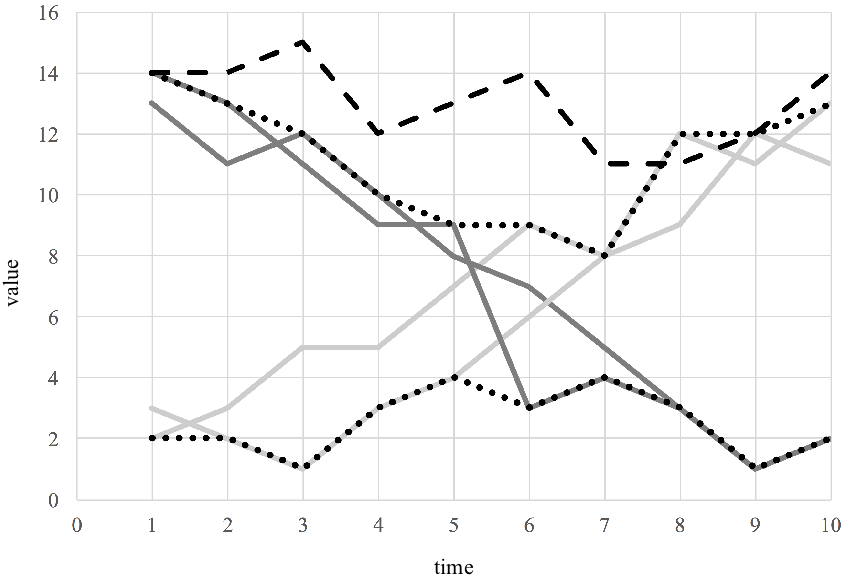
\includegraphics[scale=0.29]{figures/baseline_issue.png}
%	\caption{A possible issue of the baseline version.}
%	\label{fig:baseline_issue}
%\end{figure}

%To overcome this issue, the \ctsr clusters the time series contained within each node and then generates and stores separate upper and lower bounds for each cluster.

%Towards this, we employ the $k$-means clustering, starting from the leaf nodes of the tree and proceeding in a bottom-up fashion to the inner nodes. For each leaf node, we generate $k$ clusters of the time series contained in it, and we calculate the corresponding upper and lower bounds for each cluster. Then, we propagate them to the upper levels of the index (\mnote{TODO: elaborate}).

%Figure \ref{fig:issue_resolved} depicts this approach, where the dotted line represents the bounds for the first group and the bold dashed line represents the bounds for the second (\mnote{TODO: update}). It is obvious that the distance between the upper bounds of both groups and the query time series is rather large this time and the node containing those bounds can be more effectively pruned. 

%\begin{figure}[ht]
%	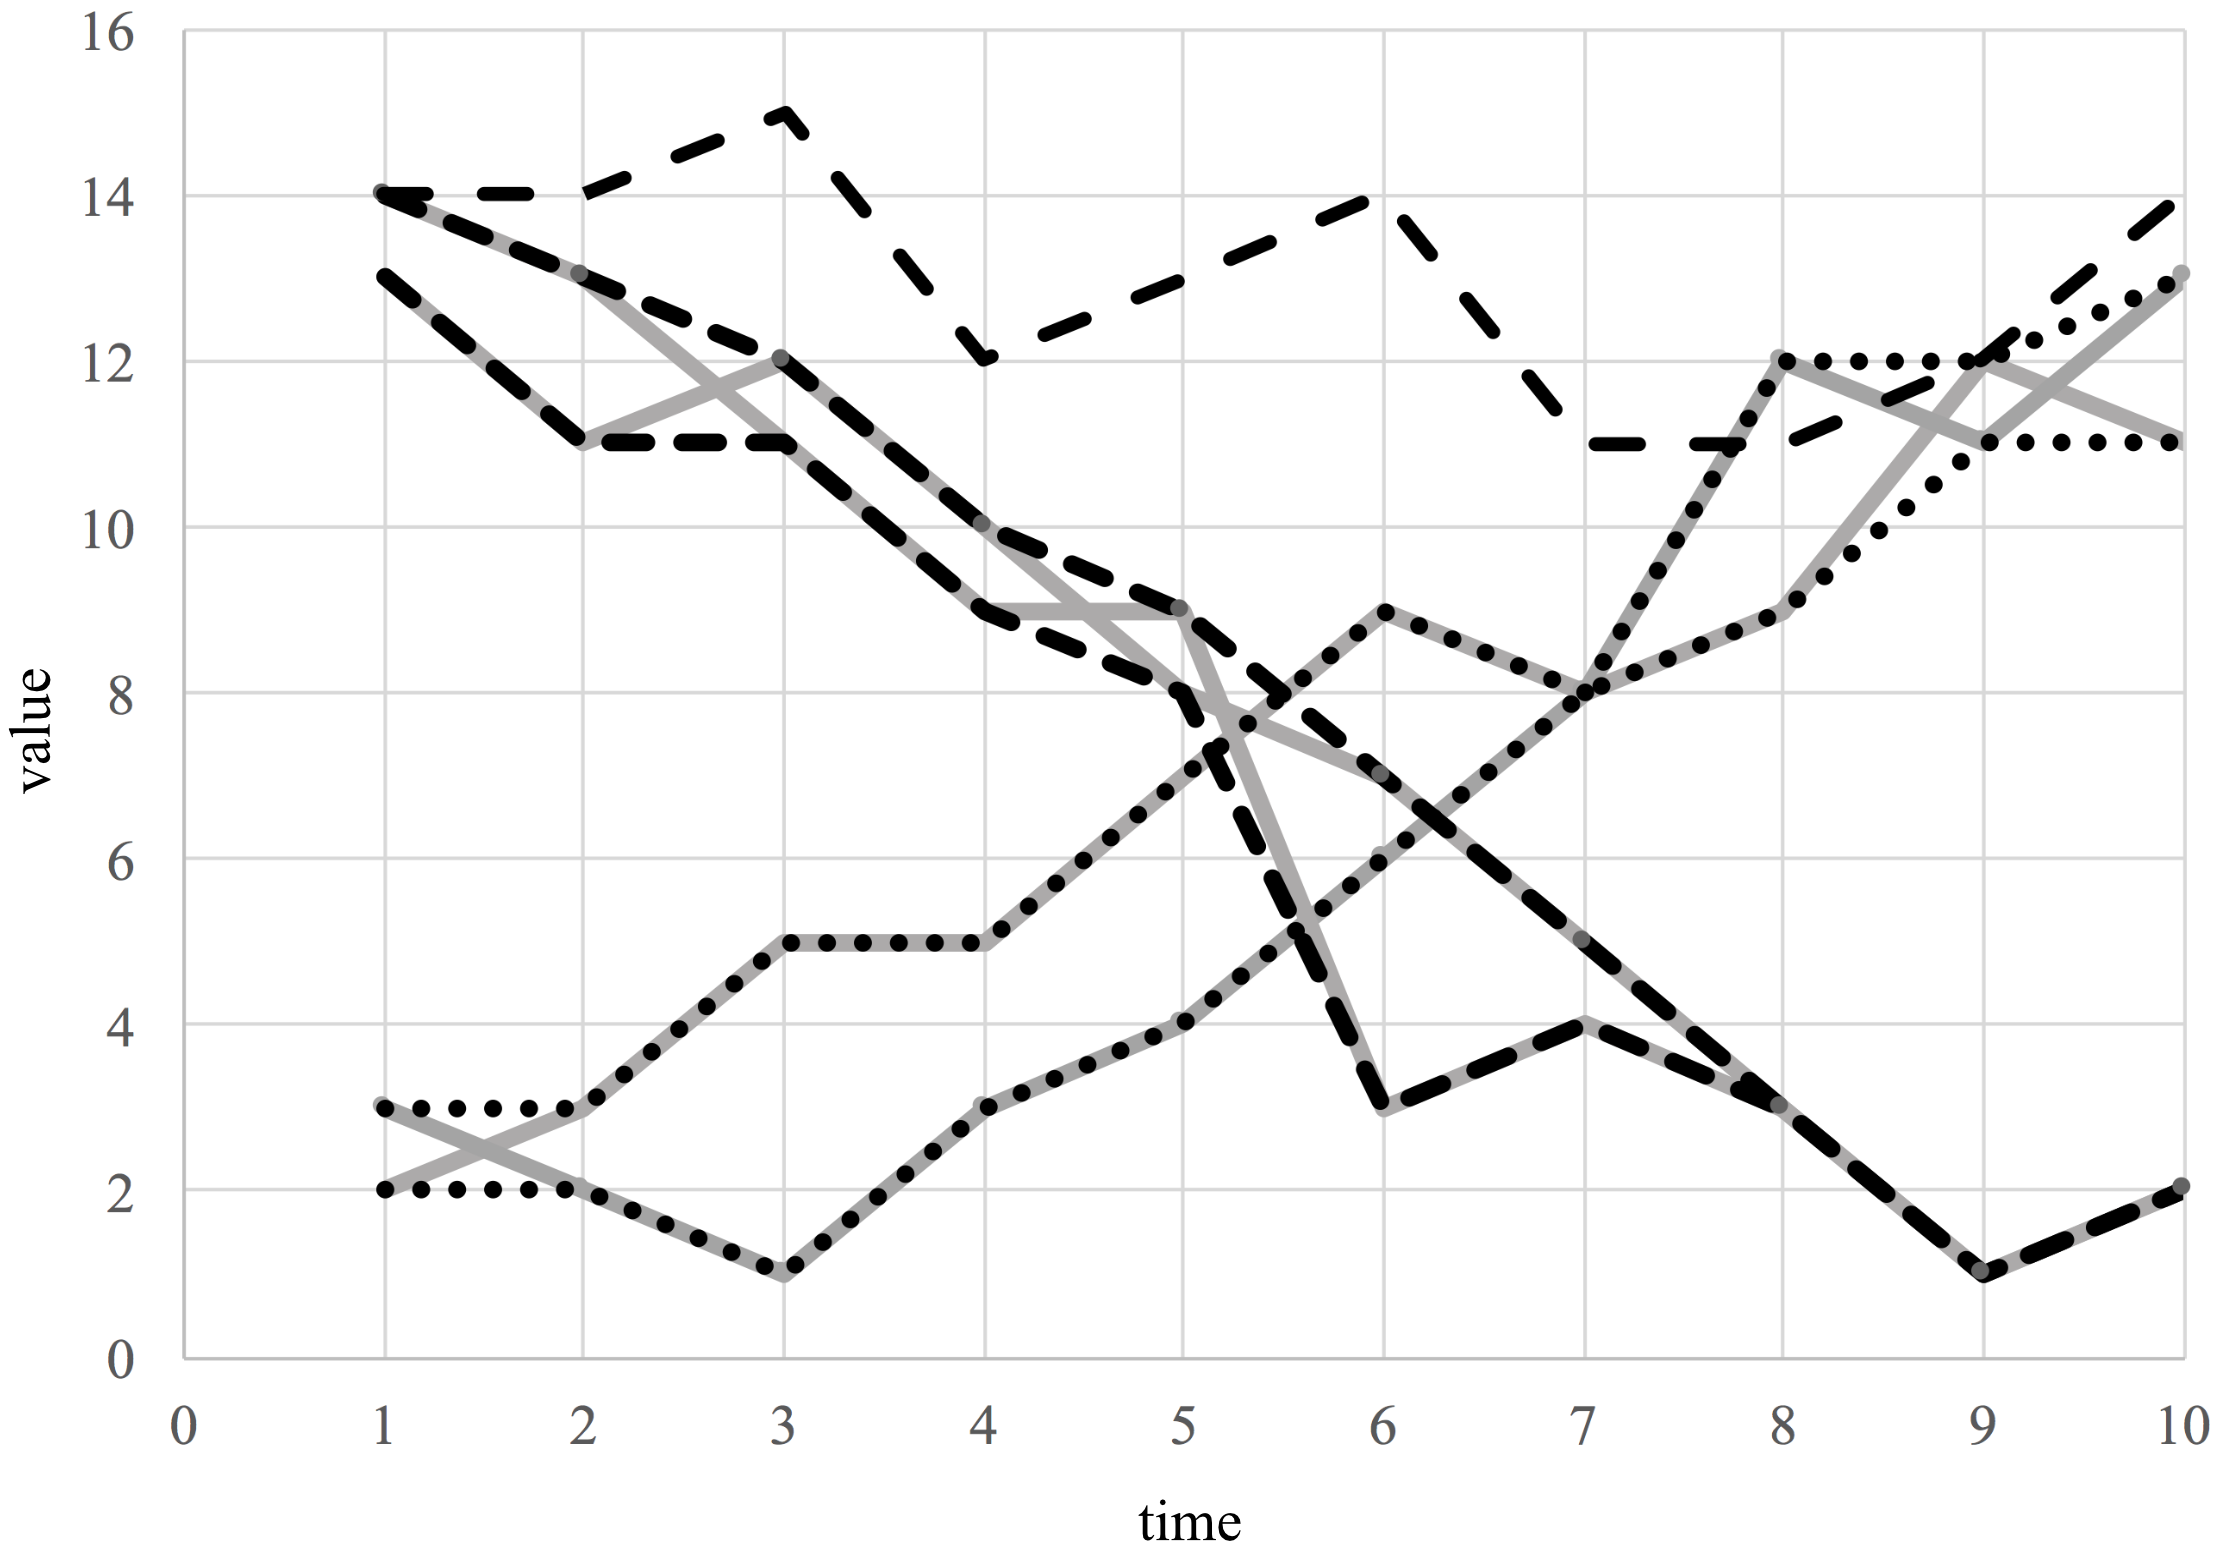
\includegraphics[scale=0.29]{figures/issue_resolved.png}
%	\caption{By clustering the time-series contained by each node we can prune even further.}
%	\label{fig:issue_resolved}
%\end{figure}

%Consequently, each node entry of the \ctsr index holds the following information:
%
%\begin{itemize}
%	\item An MBR of all its sub-trees in the spatial domain.
%	\item The average time-series word of all the time-series contained in its sub-trees.
%	\item A number of upper bounds for each cluster of time-series contained in its sub-trees.
%	\item A number of lower bounds for each cluster of time-series contained in its sub-trees.
%\end{itemize}

%In fact, its construction starts by first constructing the \tsr. Then, the process proceeds recursively from the leaf nodes to the root. Initially, for each leaf node, it executes the $k$-means algorithm to generate $k$ clusters out of the contained time series, and computes the corresponding upper and lower bounds per cluster. Then, the same procedure is performed for each parent node recursively, where at each step the $k$-means clustering is executed on the centroids of each cluster of the child nodes.

%The algorithm that constructs the bounds for each level is described in Algorithm \ref{alg:create_bounds} (\mnote{TODO:check}). Initially, we recursively traverse the index (Lines 2-4) until we reach the desired level (Line 5). Then, if the current node is a leaf (Line 6), we perform clustering on the node, using its children's geo-located time-series (Line 7) and calculate its minimum and maximum bounds per cluster (Lines 8-9). If it is a non-leaf node (Line 10), we perform clustering using its children cluster centroids (Line 11) and for each cluster, we retrieve the leafs contained in its members' sub-trees and calculate the bounds (Lines 12-14). Finally, we return the computed bounds (Line 15).

%\mnote{TODO: add a few sentences for the querying part}

%\begin{algorithm}[ht]
%	\DontPrintSemicolon
%	\KwIn{Starting node $N$, number of clusters $k$, the level to be traversed $l$}
%	\KwOut{The minimum and maximum bounds for each cluster of the given node $minB, maxB$}
%	\BlankLine
%	\Begin{
%		\If{$level>1$}{
%			\ForEach{$C : N.children$}{
%				$return(createBounds(C, l-1))$
%			}
%		}
%		\ElseIf{$l==1$}{
%			\If{N.isLeaf}{
%				$clusters \leftarrow kMeans(k, N.children)$ \\
%				\ForEach{$cl : clusters$}{
%					$minB, maxB \leftarrow calculateBounds(cl)$ \\
%				}
%			}
%			\Else{
%				$clusters \leftarrow kMeans(k, N.clustCent)$ \\
%				\ForEach{$cl : clusters$}{
%					$leafs \leftarrow getSubTreeLeafs(cl)$ \\
%					$minB, maxB \leftarrow calculateBounds(leafs)$ \\	
%				}
%			}
%			$return(minB, maxB)$
%		}
%	}
%	\caption{createBounds($root$, $l$)}
%	\label{alg:create_bounds}	
%\end{algorithm}

%\subsection{Query Processing}
%\label{subsec:query_proc}

%The R-TS index supports all the query types described in \ref{subsec:query_types}. As the index gets larger, traversing it tends to be significantly expensive, as all the nodes have to be accessed to obtain the requested results.

%To overcome this issue, we introduce a Euclidean minimum bounding distance between a reference time-series and the bounds described in the previous subsection. This distance is always smaller than the actual distance of all the time-series contained within the bounds, allowing to prune the search and at the same time, ensuring no false dismissals. For example, if we seek time-series that are closer to a reference time-series than a given threshold, we can ignore a node whose minimum distance is larger to this threshold, as all the time-series it contains are even further. The minimum distance is calculated as:
%
%\begin{equation} \label{eq:6}
%	\begin{split}
%		MINDST_{b}(T, B_{u}, B_{l}) = \sqrt{\sum_{i=1}^{w}D_{i}^{2}}, \\ D_{i} =\begin{cases}
%		 													x_{i} - b_{u,i}, & \text{if $x_{i}>b_{u,i}$}.\\
%	    													b_{u,i} - x_{i}, & \text{if $x_{i}<b_{l,i}$}. \\
%	    													0, & \text{if $b_{l,i} \leq x_{i} \leq b_{u,i}$}.
%	  \end{cases}
%	\end{split}
%\end{equation}
%
%where $T$ is a time-series with values $\{x_1, ..., x_w\}$, $B_{u}$ is a set of upper bounds, $B_{l}$ is a set of lower bounds (we know that $\forall b_{u} \in B_{u}, b_{l} \in B_{l}, b_{u} \geq b_{l}$) and $w$ is their time-series length. It is worth mentioning that the $MINDST_{b}$ only applies for time-series of the same length, which is assumed to be true from this point on. The rationale behind this bounding distance is the following: If a query point is above or beneath the bounds, then its distance from the upper or lower bound respectively contributes to the minimum distance. We know that all the corresponding points of all the time-series contained within the bounds will have a larger distance from the query point. If the point is within the bounds it does not contribute to the minimum distance (is set as zero), as it may be closer to one or more time-series contained within the bounds.

%In the following, we describe the queries that are supported by the R-TS index, defined in Section \ref{subsec:query_types}.

%\subsubsection{Double Range Query}
%\label{subsubsec:double_range}

%The double range query seeks all the time-series with spatial distance from the query point less than $\theta_{sp}$, that satisfy the $\theta_{ts}$ value. In order to achieve this, we recursively traverse the index, checking at each node whether each node's MBR is within the given range and whether its time-series $MINDST_{b}$ from the node's bounds is smaller than $\theta_{ts}$. Upon reaching a leaf that satisfies the above constraints, we check again whether the spatial- and time-series domain Euclidean distances between each of the geo-located time-series it contains and the query is less than $\theta_sp$ and $\theta_{ts}$ respectively and add it to the final results. 

%is a separate query, i.e., spatial and time-series domain are evaluated separately, and is consisted of a reference time-series, a spatial range and a threshold. The query has the following format:
%\begin{equation} \label{eq:7}
%	Q_{brange} = \{q, \theta_{sp}, \theta_{ts}\}
%\end{equation}
%where $q$ is the query's geo-located time-series, $\theta_{sp}$ is a spatial and $\theta_{ts}$ a time-series domain Euclidean distance threshold that have to be satisfied in order to accept an element as part of the answer.

%Algorithm \ref{alg:double_range_query} marks out the steps we follow in order to execute the boolean range query. If the current node is not a leaf (Line 3), we loop over its children nodes and check whether each of them satisfies the given constraints (Lines 4-5). If $MINDST_{b}$ is larger than the given threshold, we know that the time-series that reside in that child node's sub-tree will be even further, thus, we can prune it. If the constraints are satisfied, the method is called recursively (Line 6). Upon reaching a leaf node, we obtain all its geo-located time-series (Line 9) and check whether each of them satisfies the given spatial- and time-series domain constraints (Line 10). If so, we add it to the results and return (Lines 11-12).



%\subsubsection{Range-Top-$k$ Query}
%\label{subsubsec:range_topk}

%To achieve this, we employ a \textit{best-first search} approach that uses a priority queue based on the time-series domain distance from the query, to hold the elements that are read from the index. Initially the root is inserted in the queue and then, it is polled and its children nodes are checked whether their MBR is closer to the query than $\theta_{sp}$. For all the children that satisfy this constraint, we calculate their $MINDIST_{b}$ and they are pushed back in the queue. If the node that is polled is a leaf, we read all its elements, calculate the Euclidean distance between their raw time-series data and the query and push them back to the queue. If a polled element is geo-located time-series object, we check whether its spatial distance to the query is less than $\theta_{sp}$ and add it to the final results. Finally, we return the results when their number exceeds $k$.

%is also a separate query, and is consisted of a reference time-series, a spatial range and a threshold. The query has the following format:
%\begin{equation} \label{eq:8}
%	Q_{brtopk} = \{q, \theta_{sp}, k\}
%\end{equation}
%where $q$ is the query's geo-located time-series, $\theta_{sp}$ is the radius around the query where we the search is limited and $k$ is the required number of results to be returned.

%\subsubsection{$k$NN Range Query}
%\label{subsubsec:knn_range}
%
%Algorithm \ref{alg:knn_range_query}, describes the followed procedure. The differences with the boolean range-top-$k$ query can be spotted in Lines 7, 8, 14 and 18-20, where the spatial domain distance computations are replaced with time-series domain distance ones.

%and is consisted of a reference time-series, a number of nearest neighbors and a threshold. Equation \ref{eq:9} illustrates its format:
%\begin{equation} \label{eq:9}
%	Q_{bknn} = \{q, k, \theta_{ts}\}
%\end{equation}
%where $q$ represents the query's geo-located time-series, $k$ is the number of spatial nearest neighbors to be obtained and $\theta_{sp}$ is a Euclidean distance threshold that has to be satisfied in order to accept an element as part of the answer. 

%\begin{algorithm}[ht]
%	\DontPrintSemicolon
%	\KwIn{Root $R$, geo-located query $T$, number of desired results $k$, threshold $\theta_{ts}$}
%	\KwOut{All the geo-located time-series that satisfy the given constraints $res$}
%	\BlankLine
%	\Begin{
%		$res \leftarrow \emptyset$ \\
%		$kNN \leftarrow kNN \cup R$ \\
%		\While{$!kNN.isEmpty$}{
%			$m \leftarrow kNN.poll$ \\
%			\If{$m.isRaw$}{
%				$dist_{ts} \leftarrow dist_{ts}(T, m)$ \\
%				\If{$dist_{ts} \leq \theta_{ts}$}{
%					$res \leftarrow res \cup m$ \\
%				}
%				\If{$res.size == k$}{
%					$break$ \\
%				}
%			}
%			\ElseIf{$m.isLeaf$}{
%				\ForEach{$el : m.children$}{
%					$el.dist \leftarrow dist_{sp}(T.loc, el.loc)$ \\
%					$kNN \leftarrow kNN \cup el$ \\
%				}
%			}
%			\Else{
%				\ForEach{$C : m.children$}{
%					$dist_{ts} \leftarrow dist_{ts}(T, C)$ \\
%					\If{$dist_{ts} \leq \theta{ts}$}{
%						$C.dist \leftarrow dist_{sp}(T.loc, C.mbr)$ \\
%						$kNN \leftarrow kNN \cup C$ \\	
%					}
%				}
%			}
%		}
%		$return(res)$
%	}
%	\caption{$k$NNRange($R$, $T$, $k$, $\theta_{ts}$)}
%	\label{alg:knn_range_query}	
%\end{algorithm}

%\subsubsection{Hybrid Range Query}
%\label{subsubsec:hybrid_range_query}
%
%The hybrid range query operates on the hybrid distance (Equation \ref{eq:4}) described in Section \ref{subsec:preliminaries}. We initially recursively traverse the index, taking under consideration only the nodes whose hybrid distance to the query is less than $\theta_{hb}$. The hybrid distance between an inner node and the query is calculated by replacing in Equation \ref{eq:4} the spatial distance with the distance between the query and the node's MBR and the time-series distance with the $MINDST_{b}$ distance between the node's bounds and the query:
%
%%and has the following format:
%%\begin{equation} \label{eq:10}
%%	Q_{hrange} = \{q, \theta_{hb}\}
%%\end{equation}
%%where $q$ is the query as a geo-located time-series and $\theta_{hb}$ is a hybrid distance threshold that has to be satisfied in order to accept an element as part of the answer.
%
%
%\begin{equation} \label{eq:11}
%	\begin{split}
%		dist_{hb}(T, N) = \lambda \cdot \frac{dist_{sp}(T.loc, N.mbr)}{maxD_{sp}} + \\ + (1-\lambda) \cdot \frac{MINDST_{b}(T, N^{b}_{u}, N^{b}_{l})}{maxD_{ts}}
%	\end{split}
%\end{equation}
%
%where $T.loc$ is the spatial part of the query, $N.mbr$ is the current node's MBR and $N^{b}_{u}, N^{b}_{l}$ are the node's upper and lower bounds recursively. Upon reaching a leaf, the hybrid distance of each element it contains to the query is calculated and only the ones that satisfy the threshold $\theta_{hb}$ are added to the results. 
%
%Algorithm \ref{alg:hybrid_range_query} describes the above procedure. If the given node is not a leaf (Line 3), we recursively call the same method (Line 6) for all the node's children whose distance from the query satisfy $\theta_{hb}$ (Lines 4-5). When a leaf is reached, we add to the results only the geo-located time-series that satisfy $\theta_{hb}$ and return the results (Lines 8-12).
%
%\begin{algorithm}[ht]
%	\DontPrintSemicolon
%	\KwIn{Starting node $N$, geo-located query $T$, threshold $\theta_{hb}$}
%	\KwOut{All the geo-located time-series that satisfy the given constraints $res$}
%	\BlankLine
%	\Begin{
%		$res \leftarrow \emptyset$ \\
%		\If{$!N.isLeaf$}{
%			\ForEach{$C : N.children$}{
%				\If{$dist_{hb}(T, C) \leq \theta_{hb}$}{
%					$res \leftarrow res \cup HybridRange(C, T, \theta_{hb})$ \\
%				}
%			}
%			$return(res)$
%		}
%		\Else{
%			\ForEach{$el : N.children$}{
%				\If{$dist_{hb}(T, el) \leq \theta_{hb}$}{
%					$res \leftarrow res \cup el$ \\
%				}
%			}
%			$return(res)$
%		}
%	}
%	\caption{HybridRange($N$, $T$, $\theta_{hb}$)}
%	\label{alg:hybrid_range_query}	
%\end{algorithm}
%
%\subsubsection{Hybrid Top-$k$ Query}
%\label{subsubsec:hybrid_topk_query}
%
%The hybrid top-$k$ query makes use of the best-first search approach, each time traversing the node that is closer to the query in terms of the hybrid distance in Equation \ref{eq:11}. The query starts from the root node, adding all its children to a priority queue that keeps them sorted according to the hybrid distance. Then at each iteration, it polls an element from the queue and, if it is an inner-node, it similarly adds its children to the queue. If it is a leaf node, it obtains its raw geo-located time-series, calculates their hybrid distance using Equation \ref{eq:4} and adds the top-$k$ of them to the top-k queue via a local queue. When, during an iteration, a raw geo-located time-series is polled from the queue, it is added to the final results. When the size of the results reaches $k$, the results are returned. This way, the remaining unexplored nodes in the queue do not need to be traversed and are thus, pruned. 
%
%%It has the following format:
%%\begin{equation} \label{eq:12}
%%	Q_{htopk} = \{q, k\}
%%\end{equation}
%%where $q$ is the query as a geo-located time-series and $k$ is the number of elements to be retrieved. 
%
%The above procedure is described in Algorithm \ref{alg:hybrid_topk_query}. Initially, the root is added to the priority queue (Lines 2-3). As a next step, we iterate over the queue, until its empty (Line 4), each time polling its top element (Line 5). If it is a raw geo-located time-series, we calculate its hybrid distance to the query and add it to the queue (Lines 7-8). The loop breaks when the size of the queue becomes equal to $k$ (Line 10) and the queue is returned as result (Line 21). If the polled element is a leaf, we iterate over its children (raw geo-located time-series), calculate their hybrid distance to the query and add the top-$k$ of them to the queue (Lines 11-16). Finally, in case the polled element is an inner node, we obtain its children nodes, calculate their hybrid distance to the query and add them back to the queue (Lines 18-20).
%
%\begin{algorithm}[ht]{}
%	\DontPrintSemicolon
%	\KwIn{Index root $R$, geo-located query $T$, number of desired results $k$}
%	\KwOut{All the geo-located time-series that satisfy the given constraints $topkQ$}
%	\BlankLine
%	\Begin{
%		$topkQ \leftarrow topkQ \cup R$ \\
%		\While{$!topkQ.isEmpty$}{
%			$m \leftarrow topkQ.poll$ \\
%			\If{$m.isRaw$}{
%				$topkQ \leftarrow topkQ \cup m$ \\
%				\If{$topkQ.size == k$}{
%					$break$ \\
%				}
%			}
%			\ElseIf{$m.isLeaf$}{
%				\ForEach{$el : m.children$}{
%					$el.dist \leftarrow dist_{hb}(T, el)$ \\
%					$topkQ \leftarrow topkQ \cup el$ \\
%				}
%			}
%			\Else{
%				\ForEach{$C : m.children$}{
%					$C.dist \leftarrow dist_{hb}(T, C)$ \\
%					$topkQ \leftarrow topkQ \cup C$ \\	
%				}
%			}
%		}
%		$return(topkQ)$
%	}
%	\caption{HybridTop$k$($R$, $T$, $k$)}
%	\label{alg:hybrid_topk_query}	
%\end{algorithm}